\section{Distillation bounds}
\label{sec:distill}

Consider a general magic state distillation process,
\begin{equation}\label{eq:distprocess}
    \rho^{\otimes k} \xrightarrow{\E \in \O} \tau,
\end{equation}
where $n$ noisy copies of magic state $\rho$ are converted to a single-copy magic state $\tau$.
Identifying a symmetry of the distillation process responsible for leaving a state $\sigma$ invariant is equivalent with restricting the process to the $\sigma$-fragment $\O_\sigma$.

Mana is monotonic and additive in all $\sigma$-fragments as seen in~\cref{app:major}, so it provides a bound for distillation processes
\begin{equation}
    \mana{\rho} \geq \frac{1}{k} \mana{\tau}.
\end{equation}.

A new bound can be obtained in any $\sigma$-fragment by comparing the Lorenz curves of the initial and target states,
\begin{equation}\label{eq:majbound}
    L_k(\rho^{\otimes k} | \sigma) \geq L_k (\tau | \sigma),\ k=1,\dots,d^2,
\end{equation}
If the Lorenz curve of the initial state is below the target curve at any point, the process is not possible.
In general, the Wigner components of a $k$-copy state $\rho^{\otimes k}$ are calculated, along with their multiplicities, by expanding the terms in the multinomial expansion $\left( \sum_{\bm{z} \in \cal{P}_d} W_\rho(\bm{z}) \right)^n$.
This follows from the multiplicativity of the Wigner distribution.

The Strange state $\ketbra{\rm{S}}$ depicted in~\cref{fig:strange} is the simplest to analyse, since it only has two distinct components $\{ -\frac{1}{3}, \frac{1}{6} \}$, the latter with a multiplicity of 8.
Calculating the binomial expansion for the components of $\ket{S}\bra{S}^{\otimes k}$ gives $\{(-1)^j 2^{j-k} 3^{-k}\}_{0 \leq j \leq k}$ with multiplicity $8^{k-j} \binom{k}{j}$ for the $j$-th term.
This allows analytical calculation of all Lorenz curve points, hence the maximum of the $k$-copy state is
\begin{equation}\label{eq:Skmax}
    \max_k{L_k \left( \ketbra{S}^{\otimes k} \bigm| \sigma \right)} = 1 + \left(\frac{4}{3}\right)^k \sum\limits_{j: 1 \leq 2j+1 \leq k} 4^{-(2j+1)} \binom{k}{2j+1}.
\end{equation}

Consider the noisy Strange state,
\begin{equation}
    \rho_{\rm{S}}(\epsilon) = (1 - \epsilon) \ket{\rm{S}}\bra{\rm{S}} + \epsilon \sigma,
\end{equation}
in the $\sigma$-fragment $\O_\sigma$.
At noise level $\epsilon \leq \frac{3}{4}$, the Wigner distribution $\W{\rho_{\rm{S}}(\epsilon)}$ contains negativities and the state can be purified so as to obtain a single-copy state with sufficiently low $\epsilon$.
In~\cref{fig:distill}, we examine the purifying process 
\begin{equation}\label{eq:purify}
    \rho_{\rm{S}}^{\otimes k}(\epsilon_{\rm{th}}) \xrightarrow{\E \in \O_\sigma} \rho_{\rm{S}}(0.05),\ \sigma = (1-p)\ketbra{0} + p \frac{1}{3}\id
\end{equation}
with $\epsilon_{\rm{th}}$ being the noise level threshold that does not prohibit the process for given number of copies $k$ and $\sigma$-fragment, parametrised by $p$ as a mixture of the zero and the maximally mixed states.
\begin{figure}
    \centering
    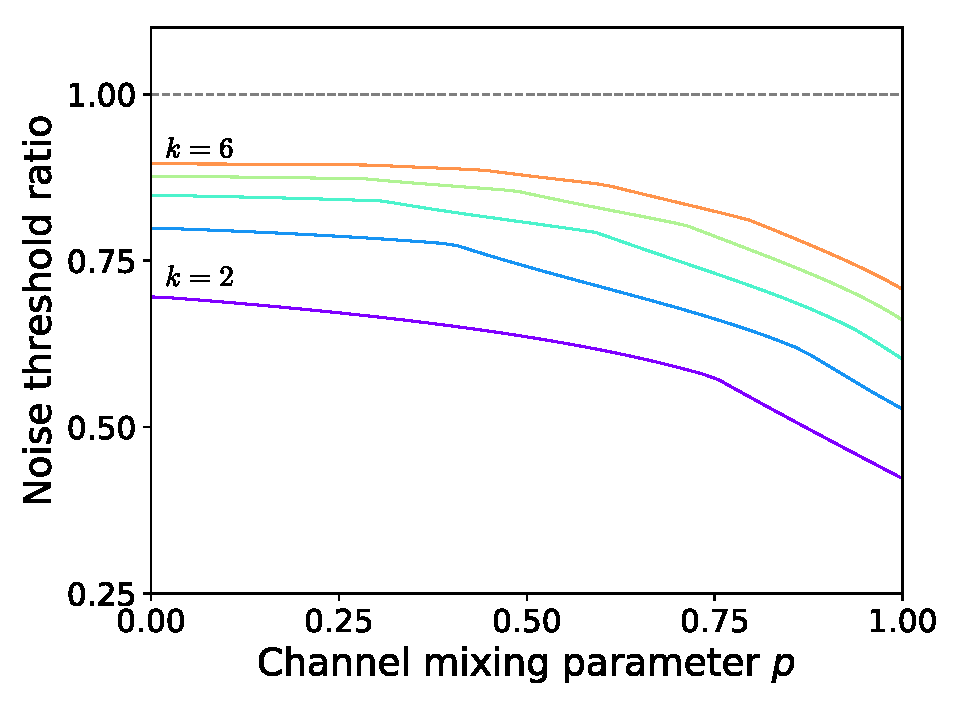
\includegraphics[scale=0.5]{sections/distill/ratios.pdf}
    \caption{Plot of the noise level threshold ratios between mana and Lorenz curve for the Strange state purifying process in~\cref{eq:purify}.
    The ratios are calculated for different numbers of initial state copies and different $\sigma$-fragments parametrised by $p$ such that $\sigma = (1-p)\ketbra{0} + p \frac{1}{3}\id$.
    Lorenz curve comparison consistently gives stricter bounds as proven in~\cref{thm:bounds}.
    }
    \label{fig:distill}
\end{figure}

Thresholds provided by Lorenz curve comparison are always much stricter than mana thresholds \nick{threshold/bound? need to define the notion of a bound precisely}.
In fact, it is clear than this is the case in any general distillation process.
\begin{theorem}\label{thm:bounds}
    Consider the distillation process in~\cref{eq:distprocess}.
    In any $\sigma$-fragment, $\W{\sigma}$-majorization provides a stricter bound than mana.
\end{theorem}
\begin{proof}
    The maximum of the Lorenz curve of a state $\rho$ can be expressed monotonically in terms of mana, independently of the $\sigma$-fragment,
    \begin{equation}
        \max_k{L_k(\rho | \sigma)} = 1 + \sum_{\bmz: \W[\bmz]{\rho}<0} \abs{\W[\bmz]{\rho}} = \frac{1}{2} \left( 1 + e^\mana{\rho} \right).
    \end{equation}
    Therefore, the majorization condition stated in~\cref{eq:majbound} implies that $\mana{\rho^{\otimes k}} \geq \mana{\tau}$.
\end{proof}